调试和测试在软件开发过程的管道中扮演着极其重要的角色。测试可以帮助我们发现问题,而调试可以修复问题。然而,如果在实现阶段遵循一定的规则,许多潜在的缺陷是可以避免的。此外,由于测试过程非常耗时,如果能够在人工测试之前使用某些工具自动分析软件,那就很好了。此外,我们应该在什么时候、如何以及对什么软件进行测试也很重要。 \par

本章中,我们将了解以下内容: \par

\begin{itemize}
	\item 了解问题的根本原因
	\item 调试C++程序
	\item 了解静态和动态分析
	\item 理解C++中的安全问题
	\item 探索单元测试、TDD和BDD
\end{itemize}

这一章中,我们将学习如何分析一个软件缺陷,如何使用GNU调试器(GDB)工具来调试程序,以及如何使用工具来自动分析软件。我们还将学习单元测试、测试驱动开发(TDD)和行为驱动开发(BDD)的概念,以及如何在软件工程开发过程中实践使用它们。 \par

\noindent\textbf{}\ \par
\textbf{代码位置} \ \par
可以从这里获取本章的源码文件:https:/​/github.​com/PacktPublishing/Expert-CPP \par

\noindent\textbf{}\ \par
\textbf{了解问题的根本原因} \ \par
在医学上,一个好的医生需要理解治疗症状和治愈疾病之间的区别。例如,给一个手臂骨折的病人止痛药只会消除症状,手术可能是帮助骨骼逐渐愈合的正确方法。 \par
根本原因分析(RCA,Root Cause Analysis)是一个系统的过程,用于识别问题的根本原因。在相关适当工具的帮助下,尝试使用一组特定的步骤来确定问题的主要原因。通过这样做,我们可以确定以下内容: \par

\begin{itemize}
	\item 发生了什么?
	\item 怎么发生的?
	\item 为什么会这样?
	\item 应该采取什么措施来防止或减少这种情况的发生,使其不再发生?
\end{itemize}

RCA假设某个操作会触发另一个操作,依此类推。通过追溯行动链的起点,我们可以发现问题的根源,以及是如何发展成我们的症状的。这正是我们应该遵循的修复或减少软件缺陷的过程。在接下来的小节中,我们将学习基本的RCA步骤,如何应用RCA过程来检测软件缺陷,以及C++开发人员应该遵循哪些规则来防止此类缺陷在软件中发生。 \par

\noindent\textbf{}\ \par
\textbf{RCA概述} \ \par
通常,RCA进程包含以下五个步骤: \par

\begin{enumerate}
	\item 确定问题:在这个阶段,我们可以找到以下问题的答案:发生了什么?问题是什么?问题是在什么环境或条件下发生?
	\item 收集数据:为了制作原因图,我们需要收集足够的数据。这个步骤可能要花费大量的时间。
	\item 制作因果图:因素图提供了一个可视化的结构,我们可以用它来组织和分析收集到的数据。因果图只不过是一个带有逻辑测试的序列图,它解释了导问题发生的事件。这一制图过程应推动数据收集过程,直到审查人员满意为止。
	\item 查询根本原因:通过检查因果图,我们可以制作一个称为根本原因图来识别问题根源的原因。
	\item 建议和解决方案:确定了根本原因,以下问题的答案可以帮助我们找到解决方案:可以做什么来防止问题再次发生?如何实施解决方案?谁将对此负责?实现解决方案的成本或风险是什么?
\end{enumerate}

RCA树图是软件工程行业中最常用的因素图之一。下面是它的一个结构示例: \par

\begin{center}
	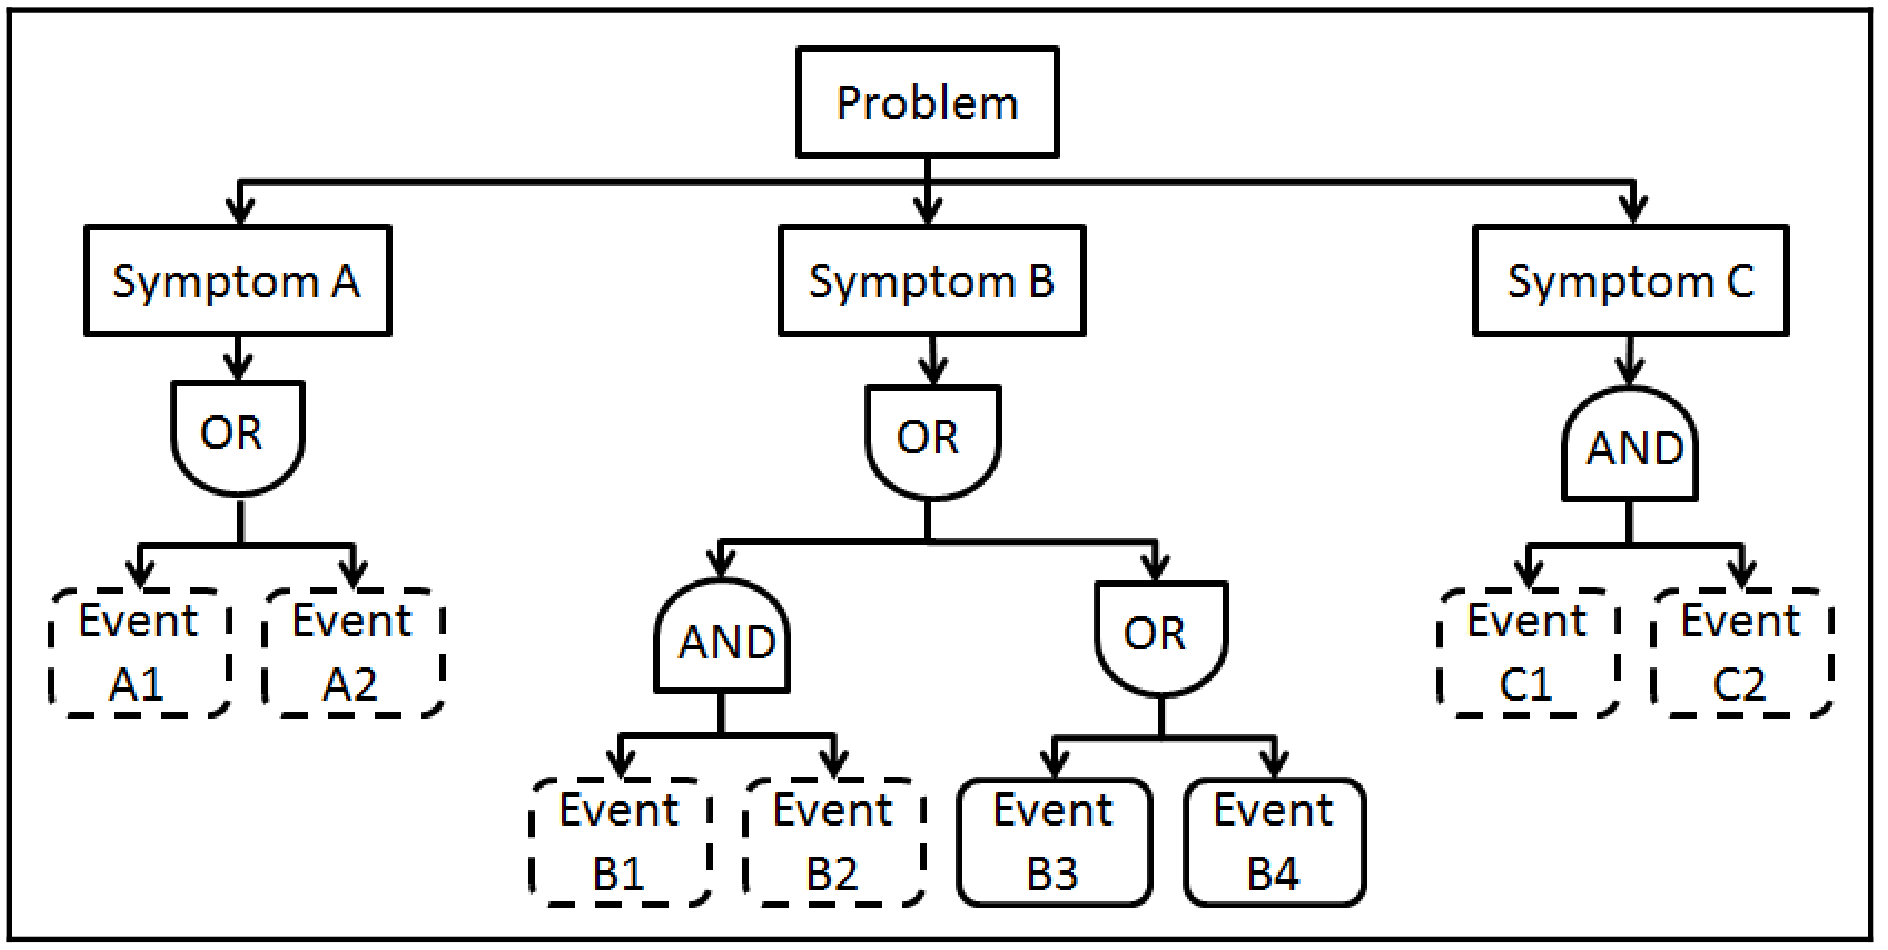
\includegraphics[width=1.0\textwidth]{content/Section-2/Chapter-13/1}
\end{center}

假设有A、B、C三种问题。现象A可以由事件A1或事件A2引起,现象B可以由事件B1和事件B2或事件B3和事件B4引起,现象C可以由事件C1和事件C2引起。数据收集后,我们发现症状A和C从未出现,B1和B2没有发生,那我们可以确定这个问题发生的原因只能是B3和B4。 \par
如果软件存在缺陷,我们应该对其应用RCA,并调查问题的根本原因,而不是在故障点上修复它。然后,问题的根本原因可以追溯到需求、设计、实现、验证和/或测试计划和输入数据。当从根本上发现并解决问题时,可以提高软件的质量,从而大大降低维护费用。 \par
我们刚刚学会了如何找到问题的根本原因,但请记住,最好的防御是进攻。所以,与其分析和解决问题,不如我们阻止它的发生? \par

\noindent\textbf{}\ \par
\textbf{防患于未然——是一种良好的编码习惯} \ \par
从成本的角度来看,IBM的研究表明,假设需求和设计的总体成本是1X,然后和编码实现过程需要5X,单元测试和集成测试需要大约10X,综合客户测试成本将~15X,修复缺陷的成本在产品发布会上占据了大约30X!因此,最小化代码缺陷是降低生产成本最有效的方法之一。 \par
尽管找到软件缺陷根本原因的通用方法非常重要,但如果我们能在实现阶段防止一些缺陷就更好了。要做到这一点,我们需要有良好的编码习惯,这意味着必须遵守某些规则。这些规则可以分为低级别和高级别。低级规则可能包括以下这些: \par

\begin{itemize}
	\item 未初始化变量
	\item 整数除法
	\item 错误地使用=而不是==
	\item 可能会将有符号变量赋值给无符号变量
	\item switch语句中缺少break
	\item 复合表达式或函数调用中的错误
\end{itemize}

当涉及到高级规则时,则为: \par

\begin{itemize}
	\item 接口
	\item 资源管理
	\item 内存管理
	\item 并发性
\end{itemize}

B. Stroustrup和H. Sutter在他们的在线文档,C++核心指南(0.8版)中建议遵循这些规则,其中强调了静态类型安全和资源安全。还强调了范围检查的可能性,以避免对空指针、悬空指针进行解引用,以及系统地使用异常。如果开发人员遵循这些规则,那么代码将是静态安全的,不会有任何资源泄漏。此外,它不仅可以捕获更多的编程逻辑错误,而且还可以运行得更快。 \par
由于页面的限制,我们将在本小节中只看几个例子。如果你想看更多的例子,请访问https:// isocpp.github.io/CppCoreGuidelines \par

\noindent\textbf{}\ \par
\textbf{未初始化变量的问题} \ \par
未初始化的变量是程序员最常犯的错误之一。当声明一个变量时,将为它分配一定数量的连续内存。如果它没有初始化,它仍然有一些值,但没有确定的方法来预测它。因此,当我们执行程序时,会出现不可预知的行为: \par

\begin{lstlisting}[caption={}]
//ch13_rca_uninit_variable.cpp
#include <iostream>
int main()
{
	int32_t x;
	// ... //do something else but not assign value to x
	if (x>0) {
		std::cout << "do A, x=" << x << std::endl;
	}
	else {
		std::cout << "do B, x=" << x << std::endl;
	}
	return 0;
}
\end{lstlisting}

代码中,当声明x时,操作系统将分配4个字节的未使用内存给它,这意味着x的值是驻留在该内存中的任何值。每次运行这个程序时,x的地址和值都可能不同。此外,一些编译器,如Visual Studio,会在Debug版本中将x的值初始化为0,但在Release版本中保持它不初始化。在这种情况下,我们在Debug和Release版本中有完全不同的输出。 \par

\noindent\textbf{}\ \par
\textbf{复合表达式中的副作用} \ \par
当运算符、表达式、语句或函数完成计算后,它可能会被延长或持续存在于其复合函数中。这种持续的存在有一些副作用,可能会导致一些不确定的行为。让我们看看下面的代码来理解这一点: \par

\begin{lstlisting}[caption={}]
//ch13_rca_compound.cpp
#include <iostream>
int f(int x, int y)
{
	return x*y;
}

int main()
{
	int x = 3;
	std::cout << f(++x, x) << std::endl; //bad,f(4,4) or f(4,3)?
}
\end{lstlisting}

由于操作数求值顺序的未定义行为,前面代码的结果可能是16或12。 \par

\noindent\textbf{}\ \par
\textbf{混合有符号和无符号的问题} \ \par
通常情况下,二元操作符 + , - ,  * ,  / ,  \% ,  < ,  <= , > , >= ,  == ,  != ,  \&\& ,  || ,  !, \&, |, <<, >>, ~, \^, =, +=, -=, *=, /=,和\%=要求两边操作数都是同一类型的。如果这两个操作数的类型不同,其中一个将隐式转换为与另一个相同的类型。[ISO/IEC 9999:2011]6.3.1.1中给出了三种C标准转换规则:\par

\begin{itemize}
	\item 当混合相同级别的类型时,有符号类型将被提升为无符号类型。
	\item 当混合不同级别的类型时,如果低级别的一方的所有值都可以由高级别的一方表示,那么低级别的一方将提升为高级别的类型。
	\item 如果在前面的情况下,低级别类型的所有值都不能用高级别类型表示,那么将使用高级别类型的无符号版本。
\end{itemize}

现在,让我们来看看传统的有符号整数减无符号整数的问题: \par

\begin{lstlisting}[caption={}]
//ch13_rca_mix_sign_unsigned.cpp
#include <iostream>
using namespace std;
int main()
{
	int32_t x = 10;
	uint32_t y = 20;
	uint32_t z = x - y; //z=(uint32_t)x - y
	cout << z << endl; //z=4294967286.
}
\end{lstlisting}

上面的例子中,有符号的int会自动转换成uint,结果是uint32\underline{ }t z = -10。另一方面,因为−10不能表示为无符号整数值,它的十六进制值0xFFFFFFF6在2的补码机器上被解释为UINT\underline{ }MAX - 9(即4294967286)。 \par

\noindent\textbf{}\ \par
\textbf{顺序问题} \ \par
下面的示例是关于构造函数中类成员的初始化顺序的。由于初始化顺序是类成员在类定义中出现的顺序,因此最好将每个成员的声明分成不同的行: \par

\begin{lstlisting}[caption={}]
//ch13_rca_order_of_evaluation.cpp
#include <iostream>
using namespace std;

class A {
public:
	A(int x) : v2(v1), v1(x) {
	};
	void print() {
		cout << "v1=" << v1 << ",v2=" << v2 << endl;
	};
protected:
	//bad: the order of the class member is confusing, better
	//separate it into two lines for non-ambiguity order declare
	int v1, v2;
};

class B {
public:
	//good: since the initialization order is: v1 -> v2,
	//after this we have: v1==x, v2==x.
	B(int x) : v1(x), v2(v1) {};
	
	//wrong: since the initialization order is: v1 -> v2,
	//after this we have: v1==uninitialized, v2==x.
	B(float x) : v2(x), v1(v2) {};
	void print() {
		cout << "v1=" << v1 << ", v2=" << v2 << endl;
	};

protected:
	int v1; //good, here the declaration order is clear
	int v2;
};
int main()
{
	A a(10);
	B b1(10), b2(3.0f);
	a.print(); //v1=10,v2=10,v3=10 for both debug and release
	b1.print(); //v1=10, v2=10 for both debug and release
	b2.print(); //v1=-858993460,v2=3 for debug; v1=0,v2=3 for release.
}
\end{lstlisting}

A类中,虽然声明顺序是v1->v2,将它们放在一行会使其他开发人员感到困惑。在B类的第一个构造函数中,v1将初始化为x,然后v2将初始化为v1,因为它的声明顺序是v1->v2。然而,在第二个构造函数中,v1将首先初始化为v2(此时v2还没有初始化!),然后v2将由x初始化。这将导致在Debug版本和Release版本中v1的输出值不同。 \par

\noindent\textbf{}\ \par
\textbf{编译时检查与运行时检查} \ \par
下面的例子展示了运行时检查(整数类型变量云的位数)可以转化到编译时检查: \par

\begin{lstlisting}[caption={}]
//check # of bits for int
//courtesy: https://isocpp.github.io/CppCoreGuidelines/CppCoreGuidelines
int nBits = 0; // don't: avoidable code
for (int i = 1; i; i <<= 1){
	++nBits;
}
if (nBits < 32){
	cerr << "int too small\n";
}
\end{lstlisting}

由于int既可以是16位也可以是32位,这取决于操作系统,因此本例无法实现。我们应该用int32\underline{ }t,或者用以下代码替换它: \par

\begin{lstlisting}[caption={}]
static_assert(sizeof(int) >= 4); //compile-time check
\end{lstlisting}

另一个例子是将最大n个整数读入一维数组: \par

\begin{lstlisting}[caption={}]
void read_into(int* p, int n); // a function to read max n integers into *p
...
int v[10];
read_into(v, 100); //bad, off the end, but the compile cannot catch this error.
\end{lstlisting}

这个问题可以通过使用span<int>来修复: \par

\begin{lstlisting}[caption={}]
void read_into( span<int> buf); // read into a range of integers
...
int v[10];
read_into(v); //better, the compiler will figure out the number of elements
\end{lstlisting}

这里的一般规则是尽可能在编译时进行分析,而不是推迟到运行时。 \par

\noindent\textbf{}\ \par
\textbf{避免内存泄漏} \ \par
内存泄漏意味着不释放已分配的动态内存。在C中,我们使用malloc()和/或calloc()来分配内存,使用free()来释放内存。在C++中,new操作符和delete或delete[]操作符用于动态地管理内存。尽管在智能指针和资源获取初始化(RAII)的帮助下可以降低内存泄漏的风险,但如果我们希望构建高质量的代码,仍然需要遵循一些规则。\par
首先,最简单的内存管理方法是不手动为代码分配内存。例如,当可以写\texttt{T x;}时,就不要写成\texttt{T* x = new T();}或\texttt{shared\underline{ }ptr<t> x(new T());}。 \par
接下来,不要使用自己的代码管理内存,如下所示: \par

\begin{lstlisting}[caption={}]
void f_bad(){
	T* p = new T() ;
	... //do something with p
	delete p ; //leak if throw or return before reaching this line
}
\end{lstlisting}

尝试使用RAII,如下所示: \par

\begin{lstlisting}[caption={}]
void f_better()
{
	std::auto_ptr<T> p(new T()) ; //other smart pointers is ok also
	... //do something with p
	//will not leak regardless whether this point is reached or not
}
\end{lstlisting}

然后,使用unique\underline{ }ptr替换shared\underline{ }ptr,除非需要共享所有权,如下所示: \par

\begin{lstlisting}[caption={}]
void f_bad()
{
	shared_ptr<Base> b = make_shared<Derived>();
	...
} //b will be destroyed at here
\end{lstlisting}

因为b是在本地使用的,而没有复制它,所以它的refcount将始终为1。这意味着我们可以使用unique\underline{ }ptr来替换它: \par

\begin{lstlisting}[caption={}]
void f_better()
{
	unique_ptr<Base> b = make_unique<Derived>();
	... //use b locally
} //b will be destroyed at here
\end{lstlisting}

最后,即使您确实需要自己动态地管理内存,如果有一个标准容器库可用,也不要手动分配内存。 \par
本节中,我们学习了如何使用RCA定位问题,以及如何通过编写最佳实践来预防问题。接下来,我们将学习如何使用调试器工具来逐行控制程序的执行,并在运行时检查变量和表达式的值。 \par

\noindent\textbf{}\ \par
\textbf{调试C++程序} \ \par
调试是发现和解决程序问题或缺陷的过程。这可能包括交互调试、数据/控制流分析以及单元和集成测试。本节中,我们只关注交互式调试,这是使用断点逐行执行源代码的过程,同时显示所使用的变量的值及其对应的内存地址。 \par

\noindent\textbf{}\ \par
\textbf{调试C/C++程序的工具} \ \par
根据开发环境,C++社区中有许多可用的工具。下面的列表显示了不同平台上受欢迎的应用程序。 \par

\begin{itemize}
	\item Linux/Unix:
	\begin{itemize}
		\item GDB: 免费的开源命令行接口(CLI)调试器。
		\item Eclipse: 免费的开源集成开发环境(IDE)。它不仅支持调试,还支持编译、分析和智能编辑。
		\item Valgrind: 开源动态分析工具,可以用于调试内存泄漏和线程bug。
		\item Affinic:为GDB、LLDB和LLVM调试器构建的商业图形用户界面(GUI)工具。
		\item DDD : 用于GDB、DBX、JDB、XDB和Python的开放源码数据显示调试器,它以图形的形式显示数据结构。
		\item GDB的Emacs模式:开源GUI工具,在使用GDB调试时,使用GNU Emacs查看和编辑源代码。
		\item KDevelop: 免费的开源IDE和调试器工具,用于编程语言,如C/ C++、Objective-C等。
		\item Nemiver: 在GNOME桌面环境中工作良好的开源工具。
		\item SlickEdit: 调试多线程和多处理器代码的好工具。
	\end{itemize}
	\item Windows:
	\begin{itemize}
		\item Visual Studio: 带有GUI的商业工具,社区版本是免费的。
		\item GDB: 在Cygwin或MinGW的帮助下,这可以在Windows上运行。
		\item Eclipse: 它的C++开发工具(CDT)可以通过工具链中的MinGW GCC编译器安装在Windows上。
	\end{itemize}
	\item macOS:
	\begin{itemize}
		\item LLDB: Xcode在macOS上的默认调试器,并支持C/ C++和Objective-C在桌面和iOS设备及其模拟器。
		\item GDB: 命令行调试器,也用于macOS和iOS系统。
		\item Eclipse: 使用GCC的免费IDE适用于macOS。
	\end{itemize}
\end{itemize}

由于GDB可以在所有平台上运行,我们将在下面的小节中向您展示如何使用GDB。 \par

\noindent\textbf{}\ \par
\textbf{GDB概述} \ \par
GDB代表GNU调试器,它允许开发人员在另一个程序执行时查看它内部发生了什么,或者在另一个程序崩溃时查看它在做什么。GDB可以做以下四件事情: \par

\begin{itemize}
	\item 启动一个程序并指定任何可能影响其行为的内容。
	\item 使程序在给定条件下停止运行。
	\item 检查当程序停止时发生了什么。
	\item 运行程序时更改变量的值。这意味着我们可以来纠正bug的影响,或者继续查找另一个bug。
\end{itemize}

注意,这里涉及两个程序:一个是GDB,而另一个是要调试的程序。由于这两个程序既可以在同一台机器上运行,也可以在不同的机器上运行,所以我们可以有以下三种类型的调试: \par

\begin{itemize}
	\item 本机调试:两个程序在同一台机器上运行。
	\item 远程调试:GDB运行在主机上,而经过调试的程序运行在远程机器上。
	\item 模拟器调试:GDB运行在主机上,而经过调试的程序运行在模拟器上。
\end{itemize}

基于编写本书时的最新版本(GDB v8.3), GDB支持的语言包括C、C++、Objective-C、Ada、Assembly、D、Fortran、Go、OpenCL、Modula-2、Pascal和Rust。 \par
因为GDB是调试行业中最先进的工具,而且很复杂,有很多功能,所以在本节中不可能了解它的所有特性。相反,我们将通过示例来研究最有用的特性。 \par

\noindent\textbf{}\ \par
\textbf{使用GDB的例子} \ \par
在练习这些例子之前,我们需要运行以下代码来检查gdb是否已经安装在我们的系统上: \par

\begin{lstlisting}[caption={}]
~wus1/chapter-13$ gdb --help
\end{lstlisting}

如果显示以下类型的信息,我们继续:\par

\begin{lstlisting}[caption={}]
This is the GNU debugger. Usage:
gdb [options] [executable-file [core-file or process-id]]
gdb [options] --args executable-file [inferior-arguments ...]

Selection of debuggee and its files:
--args Arguments after executable-file are passed to inferior
--core=COREFILE Analyze the core dump COREFILE.
--exec=EXECFILE Use EXECFILE as the executable.
...
\end{lstlisting}

否则,我们需要安装它。让我们来看看如何在不同的操作系统上安装它: \par

\begin{itemize}
	\item Debian-based Linux:
	\begin{lstlisting}[caption={}]
	~wus1/chapter-13$ sudo apt-get install build-essential
	\end{lstlisting}
	\item Redhat-based Linux:
	\begin{lstlisting}[caption={}]
	~wus1/chapter-13$sudo yum install build-essential
	\end{lstlisting}
	\item macOS:
	\begin{lstlisting}[caption={}]
	~wus1/chapter-13$brew install gdb
	\end{lstlisting}
\end{itemize}

Windows用户可以通过MinGW分发版安装GDB。macOS将需要任务门配置。 \par
然后,再次键入\texttt{gdb --help}检查是否成功安装。 \par

\noindent\textbf{}\ \par
\textbf{设置断点和检查变量值} \ \par
下面的例子中,我们将学习如何设置断点、继续、步进或步进入函数、打印变量值以及如何在gdb中使用帮助。源码如下: \par

\begin{lstlisting}[caption={}]
//ch13_gdb_1.cpp
#include <iostream>
float multiple(float x, float y);
int main()
{
	float x = 10, y = 20;
	float z = multiple(x, y);
	printf("x=%f, y=%f, x*y = %f\n", x, y, z);
	return 0;
}

float multiple(float x, float y)
{
	float ret = x + y; //bug, should be: ret = x * y;
	return ret;
}
\end{lstlisting}

正如我们在第3章中提到的,让我们在调试模式下构建这个程序,如下所示: \par
\begin{lstlisting}[caption={}]
~wus1/chapter-13$ g++ -g ch13_gdb_1.cpp -o ch13_gdb_1.out
\end{lstlisting}

注意,对于g++, -g选项意味着调试信息将包含在输出二进制文件中。如果我们运行这个程序,它将显示如下输出: \par
\begin{lstlisting}[caption={}]
x=10.000000, y=20.000000, x*y = 30.000000
\end{lstlisting}

现在,使用gdb来查看bug在哪里。为此,我们需要执行以下命令行: \par
\begin{lstlisting}[caption={}]
~wus1/chapter-13$ gdb ch13_gdb_1.out
\end{lstlisting}

我们将看到以下输出: \par
\begin{lstlisting}[caption={}]
GNU gdb (Ubuntu 8.1-0ubuntu3) 8.1.0.20180409-git
Copyright (C) 2018 Free Software Foundation, Inc.
License GPLv3+: GNU GPL version 3 or later
<http://gnu.org/licenses/gpl.html>
This is free software: you are free to change and redistribute it.
There is NO WARRANTY, to the extent permitted by law. Type "show copying"
and "show warranty" for details.
This GDB was configured as "aarch64-linux-gnu".
Type "show configuration" for configuration details.
For bug reporting instructions, please see:
<http://www.gnu.org/software/gdb/bugs/>.
Find the GDB manual and other documentation resources online at:
<http://www.gnu.org/software/gdb/documentation/>.
For help, type "help".
Type "apropos word" to search for commands related to "word"...
Reading symbols from a.out...done.
(gdb)
\end{lstlisting}

现在,让我们详细看看各种命令: \par
\begin{itemize}
	\item break和run: 如果我们输入b main或break main并按Enter,一个断点将被插入到main函数中。然后,我们可以输入run或r来开始调试程序。以下信息将显示在终端窗口中。在这里,我们可以看到我们的第一个断点在源代码的第6行,并且为了等待新命令,调试过的程序已暂停:
	\begin{lstlisting}[caption={}]
	(gdb) b main
	Breakpoint 1 at 0x8ac: file ch13_gdb_1.cpp, line 6.
	(gdb) r
	Starting program: /home/nvidia/wus1/Chapter-13/a.out
	[Thread debugging using libthread_db enabled]
	Using host libthread_db library "/lib/aarch64-linux-
	gnu/libthread_db.so.1".
	
	Breakpoint 1, main () at ch13_gdb_1.cpp:6
	6 float x = 10, y = 20;
	\end{lstlisting}
	\item next,print和quit:n或next命令将转到代码的下一行。如果该行调用了一个子程序,它不会进入子程序,而会跳过调用并将其视为单个行。如果要显示变量的值,可以使用p或print命令,后面跟着变量名。最后,如果我们想要退出gdb,可以使用q或quit命令。以下是运行这些操作后,终端窗口的输出:
	\begin{lstlisting}[caption={}]
	(gdb) n
	7 float z = multiple(x, y);
	(gdb) p z
	$1 = 0
	(gdb) n
	8 printf("x=%f, y=%f, x*y = %f\n", x, y, z);
	(gdb) p z
	$2 = 30
	(gdb) q
	A debugging session is active.
	Inferior 1 [process 29187] will be killed.
	Quit anyway? (y or n) y
	~/wus1/Chapter-13$
	\end{lstlisting}
	\item step : 现在,让我们学习如何进入multiple()函数并发现bug。为此,我们需要使用b、r和n命令重新开始,首先到达第7行。然后,我们可以使用s或step命令进入multiple()函数。接下来,我们使用n命令到达第14行和p来打印ret变量的值,它是30。\texttt{ahha the bug is at line 14!:}有一个拼写错误,即x+y,而不是x*y。下面的代码块是这些命令对应的输出:
	\begin{lstlisting}[caption={}]
	~/wus1/Chapter-13$gdb ch13_gdb_1.out
		...
		(gdb) b main
		Breakpoint 1 at 0x8ac: file ch13_gdb_1.cpp, line 6.
		(gdb) r
		The program being debugged has been started already.
		Start it from the beginning? (y or n) y
		Starting program: /home/nvidia/wus1/Chapter-13/a.out
		[Thread debugging using libthread_db enabled]
		Using host libthread_db library "/lib/aarch64-linux-
	gnu/libthread_db.so.1".
	Breakpoint 1, main () at ch13_gdb_1.cpp:6
		6 float x = 10, y = 20;
		(gdb) n
		7 float z = multiple(x, y);
		(gdb) s
		multiple (x=10, y=20) at ch13_gdb_1.cpp:14
		14 float s = x + y;
		(gdb) n
		15 return s;
		(gdb) p s
		$1 = 30
	\end{lstlisting}
	\item help : 最后,让我们学习帮助命令来结束这个小示例。当启动gdb时,我们可以使用help或h命令在其命令输入行中获取特定命令的使用信息。例如,下面的终端窗口总结了我们到目前为止所学的内容:
	\begin{lstlisting}[caption={}]
	(gdb) h b
	Set breakpoint at specified location.
	break [PROBE_MODIFIER] [LOCATION] [thread THREADNUM] [if
	CONDITION]
	PROBE_MODIFIER shall be present if the command is to be placed in
	a
	probe point. Accepted values are `-probe' (for a generic,
	automatically
	guessed probe type), `-probe-stap' (for a SystemTap probe) or
	`-probe-dtrace' (for a DTrace probe).
	LOCATION may be a linespec, address, or explicit location as
	described
	below.
	....
	(gdb) h r
	Start debugged program.
	You may specify arguments to give it.
	Args may include "*", or "[...]"; they are expanded using the
	shell that will start the program (specified by the "$SHELL"
	environment
	variable). Input and output redirection with ">", "<", or ">>"
	are also allowed.
	(gdb) h s
	Step program until it reaches a different source line.
	Usage: step [N]
	Argument N means step N times (or till program stops for another
	reason).
	(gdb) h n
	Step program, proceeding through subroutine calls.
	Usage: next [N]
	Unlike "step", if the current source line calls a subroutine,
	this command does not enter the subroutine, but instead steps over
	the call, in effect treating it as a single source line.
	(gdb) h p
	Print value of expression EXP.
	Variables accessible are those of the lexical environment of the
	selected
	stack frame, plus all those whose scope is global or an entire
	file.
	(gdb) h h
	Print list of commands.
	(gdb) h help
	Print list of commands.
	(gdb) help h
	Print list of commands.
	(gdb) help help
	Print list of commands.
	\end{lstlisting}
\end{itemize}

现在,我们已经了解了一些可以用来调试程序的基本命令。这些命令是break、run、next、print、quit、step和help。我们将在下一小节中学习函数和条件断点、观察点以及continue和finish命令。 \par

\noindent\textbf{}\ \par
\textbf{函数断点、条件断点、watchpoint以及continue和finish命令} \ \par
本例中,我们将学习如何设置函数断点、条件断点和使用continue命令。然后,我们将学习如何在不需要一步一步执行所有代码行的情况下完成一个函数调用。源代码如下: \par

\begin{lstlisting}[caption={}]
//ch13_gdb_2.cpp
#include <iostream>

float dotproduct( const float *x, const float *y, const int n);
int main()
{
	float sxx,sxy;
	float x[] = {1,2,3,4,5};
	float y[] = {0,1,1,1,1};
	
	sxx = dotproduct( x, x, 5);
	sxy = dotproduct( x, y, 5);
	printf( "dot(x,x) = %f\n", sxx );
	printf( "dot(x,y) = %f\n", sxy );
	return 0;
}

float dotproduct( const float *x, const float *y, const int n )
{
	const float *p = x;
	const float *q = x; //bug: replace x by y
	float s = 0;
	for(int i=0; i<n; ++i, ++p, ++q){
		s += (*p) * (*q);
	}
	return s;
}
\end{lstlisting}

同样,在构建并运行ch13\underline{ }gdb\underline{ }2.cpp之后,我们得到如下输出: \par

\begin{lstlisting}[caption={}]
~/wus1/Chapter-13$ g++ -g ch13_gdb_2.cpp -o ch13_gdb_2.out
~/wus1/Chapter-13$ ./ch13_gdb_2.out
dot(x,x) = 55.000000
dot(x,y) = 55.000000
\end{lstlisting}

既然点乘(x,x)和点乘(x,y)得到的结果是一样的,这里肯定有问题。现在,让我们通过学习如何在dot()函数中设置断点来调试它: \par

\begin{itemize}
	\item 函数断点:要在函数的开头设置断点,可以使用b function\underline{ }name命令。我们可以在输入过程中使用制表符联想补全。例如,我们输入以下内容:
	\begin{lstlisting}[caption={}]
		(gdb) b dot<Press TAB Key>
	\end{lstlisting}
	如果我们这样做,下面的命令行将自动弹出:
	\begin{lstlisting}[caption={}]
		(gdb) b dotproduct(float const*, float const*, int)
	\end{lstlisting}
	如果是类的成员函数,则应该包含类名,如下所示:
	\begin{lstlisting}[caption={}]
		(gdb) b MyClass::foo(<Press TAB key>
	\end{lstlisting}
	\item 条件断点:有几种设置条件断点的方法:
	\begin{lstlisting}[caption={}]
		(gdb) b f.cpp:26 if s==0 //set a breakpoint in f.cpp, line 26 if
		s==0
		(gdb) b f.cpp:20 if ((int)strcmp(y, "hello")) == 0
	\end{lstlisting}
	\item 列出和删除断点:我们设置了一些断点,就可以列出或删除它们,如下所示:
	\begin{lstlisting}[caption={}]
		(gdb) i b
		(gdb) delete breakpoints 1
		(gdb) delete breakpoints 2-5
	\end{lstlisting}
	\item 使断点无条件:由于每个断点都有一个数字,我们可以从断点中删除一个条件,如下所示:
	\begin{lstlisting}[caption={}]
		(gdb) cond 1 //break point 1 is unconditional now
	\end{lstlisting}
	\item Watchpoint:当表达式的值发生变化时,Watchpoint可以停止执行,而不必预测它可能发生在哪里(在哪一行)。观察点有三种:
	\begin{itemize}
		\item watch : 当发生写操作时,gdb将中断
		\item rwatch : 当读取发生时,gdb将中断
		\item awatch : 当发生写操作或读操作时,gdb将会中断
	\end{itemize}
	下面的代码显示了一个例子:
	\begin{lstlisting}[caption={}]
		(gdb) watch v //watch the value of variable v
		(gdb) watch *(int*)0x12345678 //watch an int value pointed by an
		address
		(gdb) watch a*b + c/d // watch an arbitrarily complex
		expression
	\end{lstlisting}
	\item continue:当我们完成了对断点处变量值的检查后,我们可以使用continue或c命令继续程序执行,直到调试器遇到断点、信号、错误或正常的进程终止。
	\item finish: 一旦进入一个函数内部,我们可能想要连续地执行它,直到它返回到调用者行。这可以使用finish命令完成。
\end{itemize}

现在,让我们把这些命令放在一起来调试ch13\underline{ }gdb\underline{ }2.cpp。我们把它分为三个部分: \par
\begin{lstlisting}[caption={}]
//gdb output of example ch13_gdb_2.out -- part 1
~/wus1/Chapter-13$ gdb ch13_gdb_2.out //cmd 1
...
Reading symbols from ch13_gdb_2.out ... done.

(gdb) b dotproduct(float const*, float const*, int) //cmd 2
Breakpoint 1 at 0xa5c: file ch13_gdb_2.cpp, line 20.
(gdb) b ch13_gdb_2.cpp:24 if i==1 //cmd 3
Breakpoint 2 at 0xa84: file ch13_gdb_2.cpp, line 24.
(gdb) i b //cmd 4
Num Type Disp Enb Address What
1 breakpoint keep y 0x0000000000000a5c in dotproduct(float const*, float
const*, int) at ch13_gdb_2.cpp:20
2 breakpoint keep y 0x0000000000000a84 in dotproduct(float const*, float
const*, int) at ch13_gdb_2.cpp:24
stop only if i==1
(gdb) cond 2 //cmd 5
Breakpoint 2 now unconditional.
(gdb) i b //cmd 6
Num Type Disp Enb Address What
1 breakpoint keep y 0x0000000000000a5c in dotproduct(float const*, float
const*, int) at ch13_gdb_2.cpp:20
2 breakpoint keep y 0x0000000000000a84 in dotproduct(float const*, float
const*, int) at ch13_gdb_2.cpp:24
\end{lstlisting}

在第一部分中,我们有以下六个命令: \par

\begin{itemize}
	\item cmd 1 : 我们以构建的可执行文件ch13\underline{ }gdb\underline{ }2,并结合参数使用gdb。简要地向我们展示了它的版本、文档和使用信息,然后告诉我们读取符号的过程已经完成,正在等待下一个命令。
	\item cmd 2 : 我们设置了一个断点函数(dotproduct())。
	\item cmd 3 : 设置了条件断点。
	\item cmd 4 : 它列出了关于断点的信息,并告诉我们有两个断点。
	\item cmd 5 : 我们将断点2设置为无条件的
	\item cmd 6 : 我们再次列出断点信息。在这一点上,我们可以看到两个断点。它们位于ch13\underline{ }gdb\underline{ }2.cpp中的第20行和第24行。
\end{itemize}

接下来,让我们看看第二部分中的gdb输出: \par

\begin{lstlisting}[caption={}]
//gdb output of example ch13_gdb_2.out -- part 2
(gdb) r //cmd 7
Starting program: /home/nvidia/wus1/Chapter-13/ch13_gdb_2.out
[Thread debugging using libthread_db enabled]
Using host libthread_db library "/lib/aarch64-linux-gnu/libthread_db.so.1".

Breakpoint 1, dotproduct (x=0x7fffffed68, y=0x7fffffed68, n=5) at
ch13_gdb_2.cpp:20
20 const float *p = x;
(gdb) p x //cmd 8
$1 = (const float *) 0x7fffffed68
(gdb) c //cmd 9
Continuing.

Breakpoint 2, dotproduct (x=0x7fffffed68, y=0x7fffffed68, n=5) at
ch13_gdb_2.cpp:24
24 s += (*p) * (*q);
(gdb) p i //cmd 10
$2 = 0
(gdb) n //cmd 11
23 for(int i=0; i<n; ++i, ++p, ++q){
(gdb) n //cmd 12

Breakpoint 2, dotproduct (x=0x7fffffed68, y=0x7fffffed68, n=5) at
ch13_gdb_2.cpp:24
24 s += (*p) * (*q);
(gdb) p s //cmd 13
$4 = 1
(gdb) watch s //cmd 14
Hardware watchpoint 3: s
\end{lstlisting}

第二部分有以下cmds: \par

\begin{itemize}
	\item cmd 7 :通过给出run命令,程序开始运行,并在第20行中的第一个断点处停止。
	\item cmd 8 : 我们打印x的值,它显示了它的地址。
	\item cmd 9 : 继续运行,将在第24行中的第二个断点处停止。
	\item cmd 10 : 输出i的值,即0
	\item cmd 11-12 :我们使用下一个命令两次。此时,执行$ s += (*p)*(*q) $语句。
	\item cmd 13 : 输出s的值,即1。
	\item cmd 14 : 打印s的值。
\end{itemize}

最后,第三部分内容如下: \par

\begin{lstlisting}[caption={}]
//gdb output of example ch13_gdb_2.out -- part 3
(gdb) n //cmd 15
Hardware watchpoint 3: s

Old value = 1
New value = 5
dotproduct (x=0x7fffffed68, y=0x7fffffed68, n=5) at ch13_gdb_2.cpp:23
23 for(int i=0; i<n; ++i, ++p, ++q){
(gdb) finish //cmd 16
Run till exit from #0 dotproduct (x=0x7fffffed68, y=0x7fffffed68, n=5) at ch13_gdb_2.cpp:23

Breakpoint 2, dotproduct (x=0x7fffffed68, y=0x7fffffed68, n=5) at
ch13_gdb_2.cpp:24
24 s += (*p) * (*q);
(gdb) delete breakpoints 1-3 //cmd 17
(gdb) c //cmd 18
Continuing.

dot(x,x) = 55.000000
dot(x,y) = 55.000000
[Inferior 1 (process 31901) exited normally]
[Inferior 1 (process 31901) exited normally]
(gdb) q //cmd 19
~/wus1/Chapter-13$
\end{lstlisting}

这本部分中,我们有以下命令: \par

\begin{itemize}
	\item cmd 15 :如果执行下一个迭代,我们将使用下一个命令来查看s的值。它表明s的旧值为1 (s=1*1),新值为5 (s=1*1+2*2)。到目前为止,一切顺利!
	\item cmd 16 : finish命令用于继续运行程序,直到它退出该函数。
	\item cmd 17 : 我们删除断点1到3。
	\item cmd 18 : 使用continue命令。
	\item cmd 19 : 我们退出gdb,回到终端窗口。
\end{itemize}

\noindent\textbf{}\ \par
\textbf{将GDB记录输出到文本文件中} \ \par
在处理长堆栈跟踪或多线程堆栈跟踪时,从终端窗口查看和分析gdb输出可能会很不方便。但是,我们可以先将整个会话或特定输出记录到一个文本文件中,然后再使用其他文本编辑器工具脱机浏览它。为此,我们需要使用以下命令: \par
\begin{lstlisting}[caption={}]
(gdb) set logging on
\end{lstlisting}

当我们执行这个命令时,gdb将把所有终端窗口的输出保存到一个名为gdb.txt的文本文件中,该文件位于当前运行的gdb文件夹中。如果我们想停止日志记录,我们可以输入以下内容: \par

\begin{lstlisting}[caption={}]
(gdb) set logging off
\end{lstlisting}

GDB的一个优点是,我们可以随心所欲地打开或关闭set logging命令,而不必担心转储文件名。这是因为所有输出都连接到gdb.txt文件中。 \par
下面是要返回ch13\underline{ }gdb\underline{ }2.out的gdb输出: \par

\begin{lstlisting}[caption={}]
~/wus1/Chapter-13$ gdb ch13_gdb_2.out //cmd 1
...
Reading symbols from ch13_gdb_2.out...done.
(gdb) set logging on //cmd 2
Copying output to gdb.txt.
(gdb) b ch13_gdb_2.cpp:24 if i==1 //cmd 3
Breakpoint 1 at 0xa84: file ch13_gdb_2.cpp, line 24.
(gdb) r //cmd 4
...
Breakpoint 1, dotproduct (x=0x7fffffed68, y=0x7fffffed68, n=5) at ch13_gdb_2.cpp:24
24 s += (*p) * (*q);
(gdb) p i //cmd 5
$1 = 1
(gdb) p s //cmd 6
$2 = 1
(gdb) finish //cmd 7
Run till exit from #0 dotproduct (x=0x7fffffed68, y=0x7fffffed68, n=5) at ch13_gdb_2.cpp:24
0x00000055555559e0 in main () at ch13_gdb_2.cpp:11
11 sxx = dotproduct( x, x, 5);
Value returned is $3 = 55
(gdb) delete breakpoints 1 //cmd 8
(gdb) set logging off //cmd 9
Done logging to gdb.txt.
(gdb) c //cmd 10
Continuing.
dot(x,x) = 55.000000
dot(x,y) = 55.000000
[Inferior 1 (process 386) exited normally]
(gdb) q //cmd 11
~/wus1/Chapter-13$ cat gdb.txt //cmd 12
\end{lstlisting}

上述代码中使用的命令如下: \par

\begin{itemize}
	\item cmd 1 : 启动gdb。
	\item cmd 2 : 我们将日志标志设置为on。此时,gdb说输出将被复制到gdb.txt文件中。
	\item cmd 3 : 设置了条件断点。
	\item cmd 4 : 我们运行程序,当程序在第24行到达条件断点时停止。
	\item cmd 5 和 cmd 6 :打印i和s的值。
	\item cmd 7 : 通过执行函数的步出命令,它显示sxx是55(在调用sxx=dotproduct(x, x, 5)),程序在sxy =dotproduct(x, y, 5)行停止。
	\item cmd 8 : 删除断点1。
	\item cmd 9 : 将日志标志设置为off。
	\item cmd 10 : 当给出了continue指令,它就会执行main函数,gdb会等待一个新命令。
	\item cmd 11 :输入q退出gdb
	\item cmd 12 : 当它返回到终端时,我们在操作系统中运行cat命令打印记录的gdb.txt文件的内容。
\end{itemize}

到目前为止,我们已经学习了足够的调试程序的GDB命令。你可能已经注意到的,这样做很耗时。有时,由于在错误的地方进行调试,情况会变得更糟。为了有效地调试,我们需要遵循正确的策略。我们将在下面的小节中讨论这个问题。 \par

\noindent\textbf{}\ \par
\textbf{实际调试策略} \ \par
由于调试是软件开发生命周期中成本最高的阶段,查找bug并修复它们是不可行的,特别是对于大型、复杂的系统。但是,也有一些策略可以在实际的过程中使用,其中一些策略如下: \par
\begin{itemize}
	\item 使用printf()或std::cout:这是很古老的方式。通过将一些信息打印到终端,我们可以检查变量的值,并执行where和when类型的日志配置文件,以便进一步分析。
	\item 使用调试器:虽然学习使用GDB类调试器工具不是一夜之间的事情,但它可以节省大量时间。所以,试着慢慢地熟悉它。
	\item 重现错误:每当在字段中报告错误时,记录运行环境和输入数据。
	\item 转储日志文件:应用程序应该将日志消息转储到一个文本文件中。当崩溃发生时,我们应该首先检查日志文件,看看是否发生了异常事件。
	\item 猜测:粗略猜测一个bug的位置,然后证明它是对的还是错的。
	\item 分而治之:即使在最坏的情况下,我们不知道有什么bug,我们仍然可以使用二分搜索策略来设置断点,然后缩小范围,最终找到它们。
	\item 简化:总是从最简化的场景开始,然后逐渐添加外围设备、输入模块等,直到可以重现错误。
	\item 源代码版本控制:如果一个bug在发布版中突然出现,但它之前运行得很好,那么首先做一个源代码树检查。可能有人做了改变!
	\item 不要放弃:有些bug真的很难定位和/或修复,特别是对于复杂的和多团队参与的系统。暂时把它们放在一边,在回家的路上重新考虑一下——这个恍然大悟的时刻可能最终会显现出来。
\end{itemize}

到目前为止,我们已经学习了使用RCA进行宏观层面的问题定位,以及可以遵循的防止问题发生的良好编码实践。此外,通过使用最先进的调试器工具(如GDB),我们可以逐行控制程序的执行,这样我们就可以在微观层面分析和修复问题。所有这些活动都是程序员集中的和手动的。是否有任何自动化工具可以帮助我们诊断程序的潜在缺陷?我们将在下一节中研究静态和动态分析。 \par

\noindent\textbf{}\ \par
\textbf{了解静态和动态分析} \ \par
我们了解了根本原因分析过程以及如何使用GDB调试缺陷。本节将讨论如何分析有执行和没有执行的程序。前者称为动态分析,后者称为静态分析。\par

\noindent\textbf{}\ \par
\textbf{静态分析} \ \par
静态分析在不执行计算机程序的情况下评估计算机程序的质量。虽然这通常可以通过自动工具和代码审查/检查来检查源代码来完成,但我们在本节中只关注自动工具。 \par
自动静态代码分析工具被设计用来根据一组或多组编码规则或准则分析一组代码。通常,人们可以互换地使用静态代码分析、静态分析或源代码分析。通过扫描所有可能的代码执行路径的整个代码库,我们可以在测试阶段之前发现大量潜在的bug。但是,它也有几个局限性,如下: \par
\begin{itemize}
	\item 会产生假阳性和假阴性报警。
	\item 只应用扫描算法内部实现的规则,其中一些规则可能会被主观解释。
	\item 无法找到在运行时环境中引入的漏洞。
	\item 会给人一种所有问题都得到解决的虚假安全感。
\end{itemize}

在商业和免费的开源类别下,大约有30个自动的C/C++代码分析工具。这些工具的名称包括Clang、Clion、CppCheck、Eclipse、Visual Studio和GNU g++,这只是其中的一些。作为例子,我们将介绍-Wall, -Weffcc++和-Wextra选项,它们内置在GNU编译器g++中: \par
\begin{itemize}
	\item -Wall : 这允许所有的编译警告,这对一些用户来说是有问题的。这些警告很容易避免或修改,即使与宏结合在一起也是如此。它还支持在C++方言选项和Objective-C/C++方言选项中描述的一些特定于语言的警告。
	\item -Wextra : 顾名思义,它检查-Wall没有检查的某些额外警告标志。以下任何情况的警告信息将被打印:
	\begin{itemize}
		\item 用<、<=、>或>=操作数将指针与整数0进行比较
		\item 一个非枚举数和一个枚举数出现在条件表达式中。
		\item 模棱两可的虚基数。
		\item 下标寄存器类型数组。
		\item 使用寄存器类型变量的地址。
		\item 派生类的复制构造函数不初始化其基类。
	\end{itemize}
	\item -Weffc++ : 它检查是否违反了Scott Meyers撰写的《Effective and more Effective c++》中建议的一些准则。这些准则包括以下内容:
	\begin{itemize}
		\item 为具有动态分配内存的类定义复制构造函数和赋值操作符。
		\item 在构造函数中初始化而不是赋值。
		\item 在基类中使析构函数为虚函数。
		\item =操作符是否返回了对*this的引用
		\item 当须返回一个对象时,不要返回引用。
		\item 区分自增和自减操作符的前缀和后缀形式。
		\item 不要重载\&\&,||,或,
	\end{itemize}
\end{itemize}

为了探索这三个选项,让我们看看下面的例子:

\begin{lstlisting}[caption={}]
//ch13_static_analysis.cpp
#include <iostream>
int *getPointer(void)
{
	return 0;
}

int &getVal() {
	int x = 5;
	return x;
}

int main()
{
	int *x = getPointer();
	if( x> 0 ){
		*x = 5;
	}
	else{
		std::cout << "x is null" << std::endl;
	}
	int &y = getVal();
	std::cout << y << std::endl;
	return 0;
}
\end{lstlisting}

首先,让我们在没有任何选择的情况下构建: \par

\begin{lstlisting}[caption={}]
g++ -o ch13_static.out ch13_static_analysis.cpp
\end{lstlisting}

这可以成功构建,但如果我们像预期的那样运行将崩溃,并带有一个段错误(核心转储)消息。 \par
接下来,让我们添加-Wall, - weffc++和-Wextra选项,并重新构建它: \par

\begin{lstlisting}[caption={}]
g++ -Wall -o ch13_static.out ch13_static_analysis.cpp
g++ -Weffc++ -o ch13_static.out ch13_static_analysis.cpp
g++ -Wextra -o ch13_static.out ch13_static_analysis.cpp
\end{lstlisting}

-Wall和-Weffc++都给了我们以下信息: \par

\begin{lstlisting}[caption={}]
ch13_static_analysis.cpp: In function ‘int& getVal()’:
ch13_static_analysis.cpp:9:6: warning: reference to local variable ‘x’
returned [-Wreturn-local-addr]
int x = 5;
 ^
\end{lstlisting}

这里,编译器抱怨说,在\texttt{int \& getVal()}函数(cpp文件的第9行)中,返回了对局部变量的引用。这将不起作用,因为一旦程序离开函数,x就是死亡了(x的生命周期仅在函数的作用域内受限)。引用死亡变量没有任何意义。\par
-Wextra给了我们以下信息: \par
\begin{lstlisting}[caption={}]
ch13_static_analysis.cpp: In function ‘int& getVal()’:
ch13_static_analysis.cpp:9:6: warning: reference to local variable ‘x’
returned [-Wreturn-local-addr]
int x = 5;
^
ch13_static_analysis.cpp: In function ‘int main()’:
ch13_static_analysis.cpp:16:10: warning: ordered comparison of pointer
with integer zero [-Wextra]
if( x> 0 ){
^
\end{lstlisting}

前面的输出显示-Wextra不仅向我们提供了来自-Wall的警告,而且还检查了我们前面提到的6个东西。在这个例子中,它警告我们在代码的第16行中有一个指针和整数0之间的比较。 \par
现在我们知道了如何在编译时使用静态分析选项,我们将通过执行程序来了解动态分析。 \par

\noindent\textbf{}\ \par
\textbf{动态分析} \ \par
动态分析是动态程序分析的缩写,它通过在真实或虚拟处理器上执行软件程序来分析软件程序的性能。与静态分析类似,动态分析也可以自动或手动完成。例如,单元测试、集成测试、系统测试和验收测试通常都是人工参与的动态分析过程。另一方面,内存调试、内存泄漏检测和概要分析工具(如IBM purify、Valgrind和Clang sanitizers)都是动态分析工具。在本小节中,我们将重点关注动态分析工具。 \par
动态分析过程包括准备输入数据、启动测试程序、收集必要的参数和分析输出等步骤。粗略地说,动态分析工具的机制是它们使用代码工具和/或模拟环境来在被分析的代码执行时执行检查。我们可以通过以下方式与程序交互: \par

\begin{itemize}
	\item 源代码插植:在编译之前,在原始源代码中插入一个特殊的代码段。
	\item 目标代码插植:一个特定的二进制代码被直接添加到可执行文件中。
	\item 编译阶段检测:通过特殊的编译器开关添加检查代码。
	\item 不会改变源代码,使用特殊的执行阶段库来检测错误。
\end{itemize}

动态分析有以下优点:
\begin{itemize}
	\item 不存在假阳性或假阴性结果,因为将检测到模型没有预测到的错误。
	\item 不需要源代码,这意味着私有代码可以由第三方组织进行测试。
\end{itemize}

动态分析的缺点如下:
\begin{itemize}
	\item 只检测与输入数据相关的路由缺陷。其他缺陷可能不会被发现。
	\item 一次只能检查一个执行路径。为了获得一个完整的报告,我们需要尽可能多地运行测试。这需要大量的计算资源。
	\item 无法检查代码的正确性。从错误的操作中得到正确的结果是可能的。
	\item 在处理器上执行不正确的代码可能会产生意想不到的结果。
\end{itemize}

现在,让我们使用Valgrind来查找下面例子中给出的内存泄漏和越界问题: \par

\begin{lstlisting}[caption={}]
//ch13_dynamic_analysis.cpp
#include <iostream>
int main()
{
	int n=10;
	float *p = (float *)malloc(n * sizeof(float));
	for( int i=0; i<n; ++i){
		std::cout << p[i] << std::endl;
	}
	//free(p); //leak: free() is not called
	return 0;
}
\end{lstlisting}

使用Valgrind进行动态分析,需要执行以下步骤:
\begin{enumerate}
	\item 首先,我们需要安装valgrind。我们可以使用下面的命令来做到这一点:
	\begin{lstlisting}[caption={}]
		sudo apt install valgrind //for Ubuntu, Debian, etc.
	\end{lstlisting}
	\item 当成功安装,我们可以通过传递可执行文件作为参数来运行valgrind,以及其他参数,如下所示:
	\begin{lstlisting}[caption={}]
		valgrind --leak-check=full --show-leak-kinds=all --track-
		origins=yes \
		--verbose --log-file=valgrind-out.txt ./myExeFile myArgumentList
	\end{lstlisting}
	\item 接下来,让我们构建这个程序,如下所示:
	\begin{lstlisting}[caption={}]
		g++ -o ch13_dyn -std=c++11 -Wall ch13_dynamic_analysis.cpp
	\end{lstlisting}
	\item 然后,我们运行valgrind,就像这样:
	\begin{lstlisting}[caption={}]
		valgrind --leak-check=full --show-leak-kinds=all --track-
		origins=yes \
		--verbose --log-file=log.txt ./ch13_dyn
	\end{lstlisting}
\end{enumerate}

最后,我们可以检查log.txt的内容。粗体和斜体表示内存泄漏的位置和大小。通过检查地址(0x4844BFC)及其对应的函数名(main()),我们可以看到这个malloc在main()函数中: \par
\begin{lstlisting}[caption={}]
.. //ignore many lines at begining
by 0x108A47: main (in /home/nvidia/wus1/Chapter-13/ch13_dyn)
==18930== Uninitialised value was created by a heap allocation
==18930== at 0x4844BFC: malloc (in /usr/lib/valgrind/vgpreload_memcheck-
arm64-linux.so)
... //ignore many lines in middle
==18930== HEAP SUMMARY:
==18930== in use at exit: 40 bytes in 1 blocks
==18930== total heap usage: 3 allocs, 2 frees, 73,768 bytes allocated
==18930==
==18930== 40 bytes in 1 blocks are definitely lost in loss record 1 of 1
==18930== at 0x4844BFC: malloc (in /usr/lib/valgrind/vgpreload_memcheck-
arm64-linux.so)
==18930==
==18930== LEAK SUMMARY:
==18930== definitely lost: 40 bytes in 1 blocks
==18930== indirectly lost: 0 bytes in 0 blocks
==18930== possibly lost: 0 bytes in 0 blocks
==18930== still reachable: 0 bytes in 0 blocks
==18930== suppressed: 0 bytes in 0 blocks
\end{lstlisting}

在这里,我们可以看到调用malloc()来在地址0x4844BFC分配一些内存。堆摘要部分指出我们在0x4844BFC处有40个字节的内存丢失。最后,泄漏摘要部分显示,肯定有一个40字节的内存丢失块。通过搜索log.txt文件中0x4844BFC的地址值,我们最终发现在原始代码中没有调用free(p)行。在取消注释这一行之后,我们重新进行valgrind分析,这样泄漏问题就不会出现在报告中了。 \par
总之,在静态和动态分析工具的帮助下,程序的潜在缺陷可以自动大大减少。然而,为了确保软件的质量,必须有人参与最终的测试和评估。现在,我们将探索软件工程中的单元测试、测试驱动开发和行为驱动开发概念。 \par

\noindent\textbf{}\ \par
\textbf{探索单元测试、TDD和BDD} \ \par
在前一节中,我们学习了自动静态和动态程序分析。本节将重点讨论涉及人的(准备测试代码)测试,这是动态分析的另一部分。它们是单元测试、测试驱动开发和行为驱动开发。 \par
单元测试假定,如果我们已经有了单个代码单元,那么我们需要编写一个测试驱动程序,并准备输入数据,以检查其输出是否正确。在那之后,我们执行集成测试来测试多个单元,然后是验收测试,测试整个应用程序。由于集成和验收测试比单元测试更难维护,而且与项目更相关,所以在本书中介绍它们非常具有挑战性。\\感兴趣的同学可以登录https://www.iso.org/standard/45142.html了解更多信息。 \par
与单元测试不同,TDD认为我们应该先测试代码和数据,开发一些代码并使其快速通过,最后重构直到客户满意。另一方面,BDD的理念是我们不应该测试程序的实现,而应该测试它想要的行为。为此,BDD强调,还应该建立软件生产人员之间的交流平台和语言。 \par
我们将在下面的小节中详细讨论这些方法。 \par

\noindent\textbf{}\ \par
\textbf{单元测试} \ \par
单元是更大或更复杂的应用程序中的单个组件。通常,一个单元有它自己的用户接口,比如一个函数,一个类,或者一个完整的模块。单元测试是一种软件测试方法,用于确定代码单元是否按照其设计需求的预期行为。单元测试的主要特点如下: \par

\begin{itemize}
	\item 它小巧而简单,编写和运行速度很快,因此,它可以在开发周期的早期发现问题,因此可以很容易地修复这些问题。
	\item 因为它与依赖项隔离,所以每个测试用例都可以并行运行。
	\item 单元测试驱动程序帮助我们理解单元接口。
	\item 在集成测试单元时,会极大地帮助集成和验收测试。
	\item 通常由开发人员准备和执行。
\end{itemize}

虽然我们可以从头开始编写单元测试包,但是社区中已经开发了很多单元测试框架(UTFs)。提振。Test、CppUnit、GoogleTest、Unit++和CxxTest是最流行的。这些UTFs通常有以下特性:\par

\begin{itemize}
	\item 只需要少量的工作来设置一个新的测试。
	\item 依赖于标准库并支持跨平台,很容易移植和修改。
	\item 支持测试固件,这允许我们为多个不同的测试重用对象的相同配置。
	\item 能很好地处理异常和崩溃。这意味着UTF可以报告异常,但不能报告崩溃。
	\item 有很好的断言功能。每当断言失败时,应该打印它的源代码位置和变量的值。
	\item 支持不同的输出,这些输出可以方便地由人工或工具进行分析。
	\item 支持测试套件,每个套件可能包含几个测试用例。
\end{itemize}

现在,让我们看一个Boost UTF的示例(从v1.59.0开始)。它支持三种不同的使用变体:仅头库、静态库和共享库。它包括四种类型的测试用例:没有参数的测试用例、数据驱动的测试用例、模板测试用例和参数化测试用例。 \par
它还有七种类型的检查工具:
\begin{itemize}
	\item BOOST\underline{ }TEST()
	\item BOOST\underline{ }CHECK()
	\item BOOST\underline{ }REQUIRE()
	\item BOOST\underline{ }ERROR()
	\item BOOST\underline{ }FAIL()
	\item BOOST\underline{ }CHECK\underline{ }MESSAGE()
	\item BOOST\underline{ }CHECK\underline{ }EQUAL()。
\end{itemize}

它还以多种方式支持fixture和控制测试输出。在编写测试模块时,我们需要遵循以下原则: \par

\begin{enumerate}
	\item 定义我们的测试程序的名称。这将在输出消息中使用。 
	\item 请选择一个用法变体:仅头文件,链接静态库,或作为共享库。 
	\item 选择并向测试套件添加测试用例。  
	\item 对测试代码执行正确性检查。
	\item 在每个测试用例之前初始化测试代码。 
	\item 定制报告测试失败的方式。
	\item 控制构建测试模块的运行时行为,也称为运行时配置。
\end{enumerate}

例如,下面的示例将介绍步骤1-4。如果你有兴趣,你可以在\\https://www.boost.org/doc/libs/1\underline{ }70\underline{ }0/libs/test/doc/html/\\上获得步骤5-7的例子: \par

\begin{lstlisting}[caption={}]
//ch13_unit_test1.cpp
#define BOOST_TEST_MODULE my_test //item 1, "my_test" is module name
#include <boost/test/included/unit_test.hpp> //item 2, header-only

//declare we begin a test suite and name it "my_suite "
BOOST_AUTO_TEST_SUITE( my_suite )

//item 3, add a test case into test suit, here we choose
// BOOST_AUTO_TEST_CASE and name it "test_case1"
BOOST_AUTO_TEST_CASE(test_case1) {
	char x = 'a';
	BOOST_TEST(x); //item 4, checks if c is non-zero
	BOOST_TEST(x == 'a'); //item 4, checks if c has value 'a'
	BOOST_TEST(x == 'b'); //item 4, checks if c has value 'b'
}

//item 3, add the 2nd test case
BOOST_AUTO_TEST_CASE( test_case2 )
{
	BOOST_TEST( true );
}

//item 3, add the 3rd test case
BOOST_AUTO_TEST_CASE( test_case3 )
{
	BOOST_TEST( false );
}

BOOST_AUTO_TEST_SUITE_END() //declare we end test suite
\end{lstlisting}

为此,我们可能需要安装boost,如下所示: \par

\begin{lstlisting}[caption={}]
sudo apt-get install libboost-all-dev
\end{lstlisting}

然后,我们可以构建并运行它,如下所示: \par

\begin{lstlisting}[caption={}]
~/wus1/Chapter-13$ g++ -g c
\end{lstlisting}

上述代码的结果如下: \par

\begin{lstlisting}[caption={}]
Running 3 test cases...
ch13_unit_test1.cpp(13): error: in "my_suite/test_case1": check x == 'b'
has failed ['a' != 'b']
ch13_unit_test1.cpp(25): error: in "my_suite/test_case3": check false has
failed
*** 2 failures are detected in the test module "my_test"
\end{lstlisting}

这里,我们可以看到test\underline{ }case1和test\underline{ }case3中有失败。特别是,在test\underline{ }case1中,x的值不等于b,而且很明显,检查不能通过test\underline{ }case3中的测试。 \par

\noindent\textbf{}\ \par
\textbf{TDD} \ \par
如下图所示,TDD流程首先编写失败的测试代码,然后添加/修改代码,让测试通过。在那之后,我们重构测试计划并编写代码,直到所有的需求都得到满足。让我们来看看下面的图表: \par

\begin{center}
	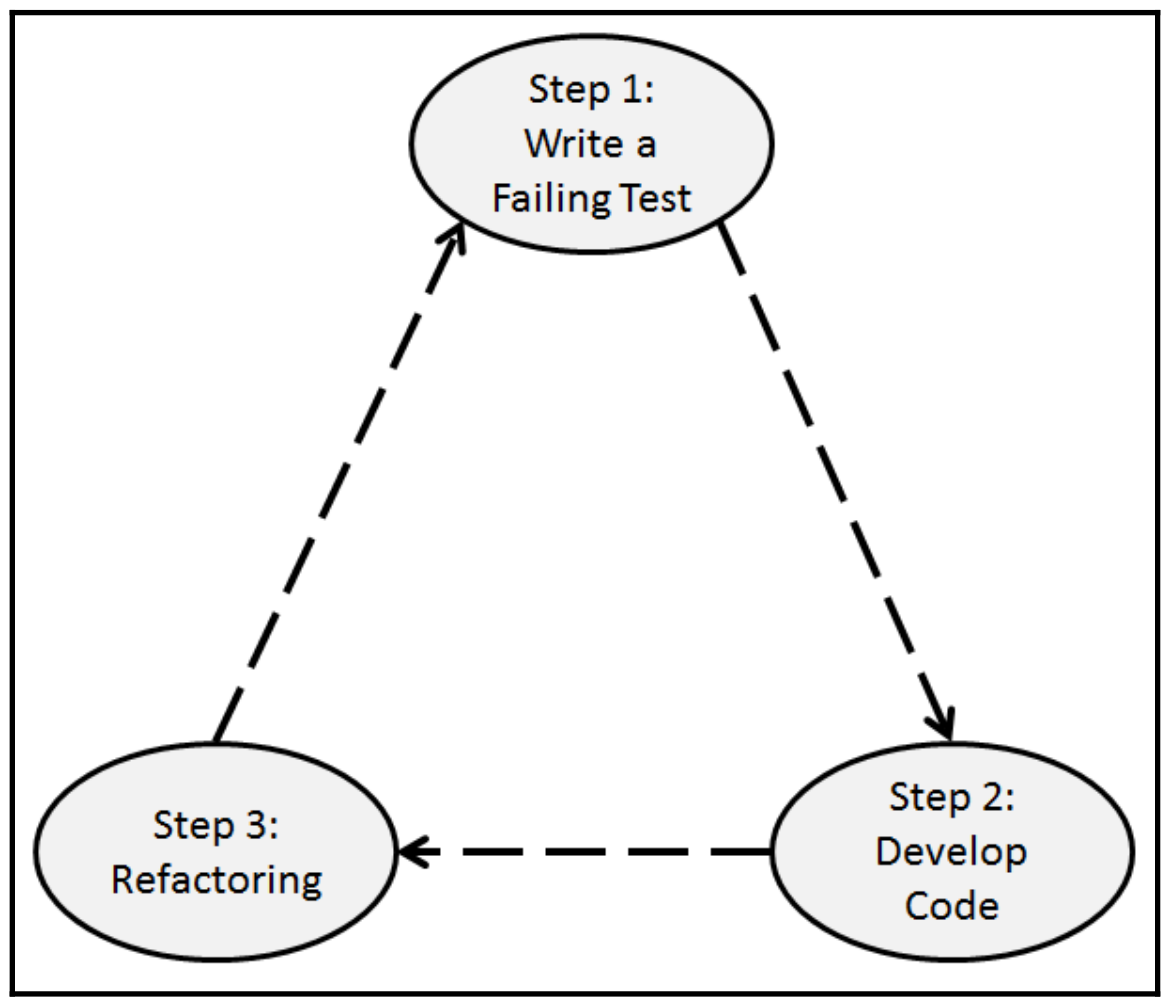
\includegraphics[width=0.6\textwidth]{content/Section-2/Chapter-13/2}
\end{center}

第1步是编写一个失败的测试。TDD不是首先开发代码,而是首先开始编写测试代码。因为我们还没有代码,所以我们知道,如果我们运行测试,它将会失败。在这一阶段,定义测试数据格式和接口,并设想代码实现细节。 \par
第2步的目标是用最少的开发工作使测试尽可能快地通过。我们不想完美地实现每件事,我们只想让它通过测试。一旦它变成绿色,我们就有东西可以展示和告诉客户,这时客户可能会在看到最初的产品后改进需求。然后,我们进入下一阶段。 \par
第三个阶段是重构。在这一阶段,我们可能会走进去,看看我们想要改变什么,以及如何改变它。\par
对于传统的开发人员来说,TDD最困难的事情就是从“编码->测试”模式转变为“测试->编码”模式。为了对测试套件有一个模糊的概念,J. Hartikainen建议开发人员从一开始考虑以下五个步骤: \par

\begin{enumerate}
	\item 首先决定输入和输出。
	\item 选择类/函数签名。 
	\item 只决定要测试的功能的一个微小方面。
	\item 实现测试。
	\item 实现的代码。
\end{enumerate}

当我们完成了这个迭代,我们就可以逐步重构它,直到实现了整体的全面目标。 \par

\noindent\textbf{}\ \par
\textbf{TDD的例子} \ \par
接下来,我们将通过一个案例研究的实现来演示TDD过程。过程中中,我们将开发一个Mat类来执行二维矩阵代数,就像我们在Matlab中所做的那样。这是一个类模板,可以保存所有数据类型的$ m × n $矩阵。矩阵代数包括矩阵的加、减、乘、除,还具有元素运算能力。 \par
让我们开始吧! \par

\noindent\textbf{}\ \par
\textbf{步骤1 -编写一个失败的测试} \ \par
首先,我们只需要以下内容: \par
\begin{enumerate}
	\item 根据给定的行数和cols创建一个Mat对象(默认值应该是$ 0 × 0 $,这是一个空矩阵)。
	\item 逐行打印它的元素。
	\item 从rows()和cols()中获取矩阵大小
\end{enumerate}

基于这些需求,我们可以有失败的单元测试代码来增强UTF,如下所示: \par

\begin{lstlisting}[caption={}]
// ch13_tdd_boost_UTF1.cpp
#define BOOST_TEST_MODULE tdd_test
#include <boost/test/included/unit_test.hpp>
#include "ch13_tdd_v1.h"

BOOST_AUTO_TEST_SUITE(tdd_suite) //begin a test suite: "tdd_suite"

BOOST_AUTO_TEST_CASE(test_case1) {
	Mat<int> x(2, 3); //create a 2 x 3 int matrix
	x.print("int x=");
	BOOST_TEST(2 == x.rows());
	BOOST_TEST(3 == x.cols());
	
	Mat<float> y; //create a 0 x 0 empty float matrix
	y.print("float y=");
	BOOST_TEST(0 == y.rows());
	BOOST_TEST(0 == y.cols());
	
	Mat<char> z(1,10); //create a 1 x 10 char matrix
	z.print("char z=");
	BOOST_TEST(1 == z.rows());
	BOOST_TEST(10 == z.cols());
}
BOOST_AUTO_TEST_SUITE_END() //end test suite
\end{lstlisting}

既然我们的测试代码已经准备好了,我们就可以开发代码了。 \par

\noindent\textbf{}\ \par
\textbf{步骤2 -开发代码让测试通过} \ \par
实现最小代码段的一种方法是通过前面的测试,如下所示: \par

\begin{lstlisting}[caption={}]
//file: ch13_tdd_v1.h
#ifndef __ch13_TDD_V1__
#define __ch13_TDD_V1__
#include <iostream>
#include <assert.h>
template< class T>
class Mat {
	public:
	Mat(const uint32_t m=0, const uint32_t n=0);
	Mat(const Mat<T> &rhs) = delete;
	~Mat();
	
	Mat<T>& operator = (const Mat<T> &x) = delete;
	
	uint32_t rows() { return m_rows; }
	uint32_t cols() { return m_cols; }
	void print(const char* str) const;
	
private:
	void creatBuf();
	void deleteBuf();
	uint32_t m_rows; //# of rows
	uint32_t m_cols; //# of cols
	T* m_buf;
};
#include "ch13_tdd_v1.cpp"
#endif
\end{lstlisting}

我们有了前面的头文件,就可以开发它对应的cpp,如下所示: \par

\begin{lstlisting}[caption={}]
//file: ch13_tdd_v1.cpp
#include "ch13_tdd_v1.h"
using namespace std;

template< class T>
Mat<T>::Mat(const uint32_t m, const uint32_t n)
: m_rows(m)
, m_cols(n)
, m_buf(NULL)
{
	creatBuf();
}

template< class T>
Mat<T> :: ~Mat()
{
	deleteBuf();
}

template< class T>
void Mat<T>::creatBuf()
{
	uint32_t sz = m_rows * m_cols;
	if (sz > 0) {
		if (m_buf) { deleteBuf();}
		m_buf = new T[sz];
		assert(m_buf);
	}
	else {
		m_buf = NULL;
	}
}

template< class T>
void Mat<T>::deleteBuf()
{
	if (m_buf) {
		delete[] m_buf;
		m_buf = NULL;
	}
}

template< class T>
void Mat<T> ::print(const char* str) const
{
	cout << str << endl;
	cout << m_rows << " x " << m_cols << "[" << endl;
	const T *p = m_buf;
	for (uint32_t i = 0; i<m_rows; i++) {
		for (uint32_t j = 0; j < m_cols; j++) {
			cout << *p++ << ", ";
		}
		cout << "\n";
	}
	cout << "]\n";
}
\end{lstlisting}

假设我们使用g++来构建和执行它,g++支持\texttt{-std=c++11}或更高版本: \par

\begin{lstlisting}[caption={}]
~/wus1/Chapter-13$ g++ -g ch13_tdd_boost_UTF1.cpp
~/wus1/Chapter-13$ a.out
\end{lstlisting}

输出如下: \par

\begin{lstlisting}[caption={}]
Running 1 test case...
	int x=2 x 3[
	1060438054, 1, 4348032,
	0, 4582960, 0,
	]
	float y=0 x 0[
	]
	char z=1 x 10[
	s,s,s,s,s,s,s,s,s,s,
	]
\end{lstlisting}

在test\underline{ }case1中,我们创建了三个矩阵,并测试了rows()、cols()和print()函数。第一个是一个2x3的int型矩阵。由于它没有初始化,其元素的值是未知的,这就是为什么我们可以从print()中看到这些随机数。此时我们还传递了rows()和cols()测试(两次BOOST\underline{ }TEST()调用都没有错误)。第二个是一个空的浮点型矩阵,它的print()函数什么也不给出,cols()和rows()都是零。最后,第三个是一个1x10的char类型未初始化矩阵。同样,这三个函数的所有输出都符合预期。 \par

\noindent\textbf{}\ \par
\textbf{步骤3 -重构} \ \par
目前为止,一切顺利——我们通过了测试!但是,在将上述结果显示给我们的客户后,他/她可能会要求我们再增加两个接口,例如: \par

\begin{itemize}
	\item 为所有元素创建一个具有给定初始值的$ m $x $n $矩阵。
	\item 添加numel()返回矩阵的元素总数。
	\item 添加empty(),如果矩阵的行数为零或列数为零,则返回true,否则返回false。
\end{itemize}

当将第二个测试用例添加到测试套件中,整个重构的测试代码如下: \par

\begin{lstlisting}[caption={}]
// ch13_tdd_Boost_UTF2.cpp
#define BOOST_TEST_MODULE tdd_test
#include <boost/test/included/unit_test.hpp>
#include "ch13_tdd_v2.h"

//declare we begin a test suite and name it "tdd_suite"
BOOST_AUTO_TEST_SUITE(tdd_suite)

//add the 1st test case
BOOST_AUTO_TEST_CASE(test_case1) {
	Mat<int> x(2, 3);
	x.print("int x=");
	BOOST_TEST(2 == x.rows());
	BOOST_TEST(3 == x.cols());
	
	Mat<float> y;
	BOOST_TEST(0 == y.rows());
	BOOST_TEST(0 == y.cols());
	
	Mat<char> z(1, 10);
	BOOST_TEST(1 == z.rows());
	BOOST_TEST(10 == z.cols());
}

//add the 2nd test case
BOOST_AUTO_TEST_CASE(test_case2)
{
	Mat<int> x(2, 3, 10);
	x.print("int x=");
	BOOST_TEST( 6 == x.numel() );
	BOOST_TEST( false == x.empty() );
	Mat<float> y;
	BOOST_TEST( 0 == y.numel() );
	BOOST_TEST( x.empty() ); //bug x --> y
}

BOOST_AUTO_TEST_SUITE_END() //declare we end test suite
\end{lstlisting}

下一步是修改代码以通过这个新测。简单起见,我们在这里不展示ch13\underline{ }tdd\underline{ }v2.h和ch13\underline{ }tdd\underline{ }v2.cpp文件。可以从本书的GitHub存储库中下载它们。在构建并执行ch13\underline{ }tdd\underline{ }Boost\underline{ }UTF2.cpp之后,我们得到如下输出: \par

\begin{lstlisting}[caption={}]
Running 2 test cases...
	int x=2x3[
	1057685542, 1, 1005696,
	0, 1240624, 0,
	]
	int x=2x3[
	10, 10, 10,
	10, 10, 10,
	]
	../Chapter-13/ch13_tdd_Boost_UTF2.cpp(34): error: in
	"tdd_suite/test_case2": che
	 ck x.empty() has failed [(bool)0 is false]
\end{lstlisting}

第一个输出中,因为我们只是定义了一个2x3的整数矩阵,并且没有在test\underline{ }case1中初始化它,所以将输出未定义的行为——即6个随机数。第二个输出来自test\underline{ }case2,其中x的所有6个元素都初始化为10。在我们对前面的结果进行了展示和说明之后,我们的客户可能会要求我们添加其他新功能或修改当前现有的功能。经过几次迭代,最终,我们将到达满意点并停止分解。 \par
现在我们已经了解了TDD,我们将来了解BDD。 \par

\noindent\textbf{}\ \par
\textbf{BDD} \ \par
软件开发中最困难的部分是与业务参与者、开发人员和质量分析团队进行沟通。一个项目很容易超出预算,错过最后期限,或者因为误解或模糊的需求、技术争论和缓慢的反馈周期而完全失败。 \par
BDD是一个敏捷开发过程,它包含一组实践,旨在减少沟通差距/障碍和其他浪费的活动。它还鼓励团队成员在生产生命周期中不断地与真实的示例进行交流。 \par
BDD包含两个主要部分:问题发现和TDD。为了让不同组织和团队中的人理解所开发软件的正确行为,有意的在发现阶段引入了一个示例映射技术,使不同角色的人通过具体的示例进行对话。这些例子将成为系统行为的自动化测试和活生生的文档。在TDD阶段,BDD指定任何软件单元的测试都应该根据单元的期望行为来指定。 \par
有几种针对不同平台和编程语言的BDD框架工具(JBehave、RBehave、Fitnesse、Cucumber等)。一般来说,这些框架执行以下步骤: \par

\begin{enumerate}
	\item 阅读业务分析人员在有意发现阶段准备的规范格式文档。
	\item 将文档转换成有意义的子句。每个单独的子句都可以设置到QA的测试用例中。开发人员也可以从子句实现源代码。
	\item 自动为每个子句场景执行测试。
\end{enumerate}

总之,我们已经了解了应用程序开发管道中应该涉及什么、何时、如何以及测试过程的策略。如下图所示,传统的v形模型强调需求模式->设计->编码->测试。TDD认为开发过程应该由测试驱动,而BDD将不同背景和角色的人之间的交流添加到TDD框架中,侧重于行为测试: \par

\begin{center}
	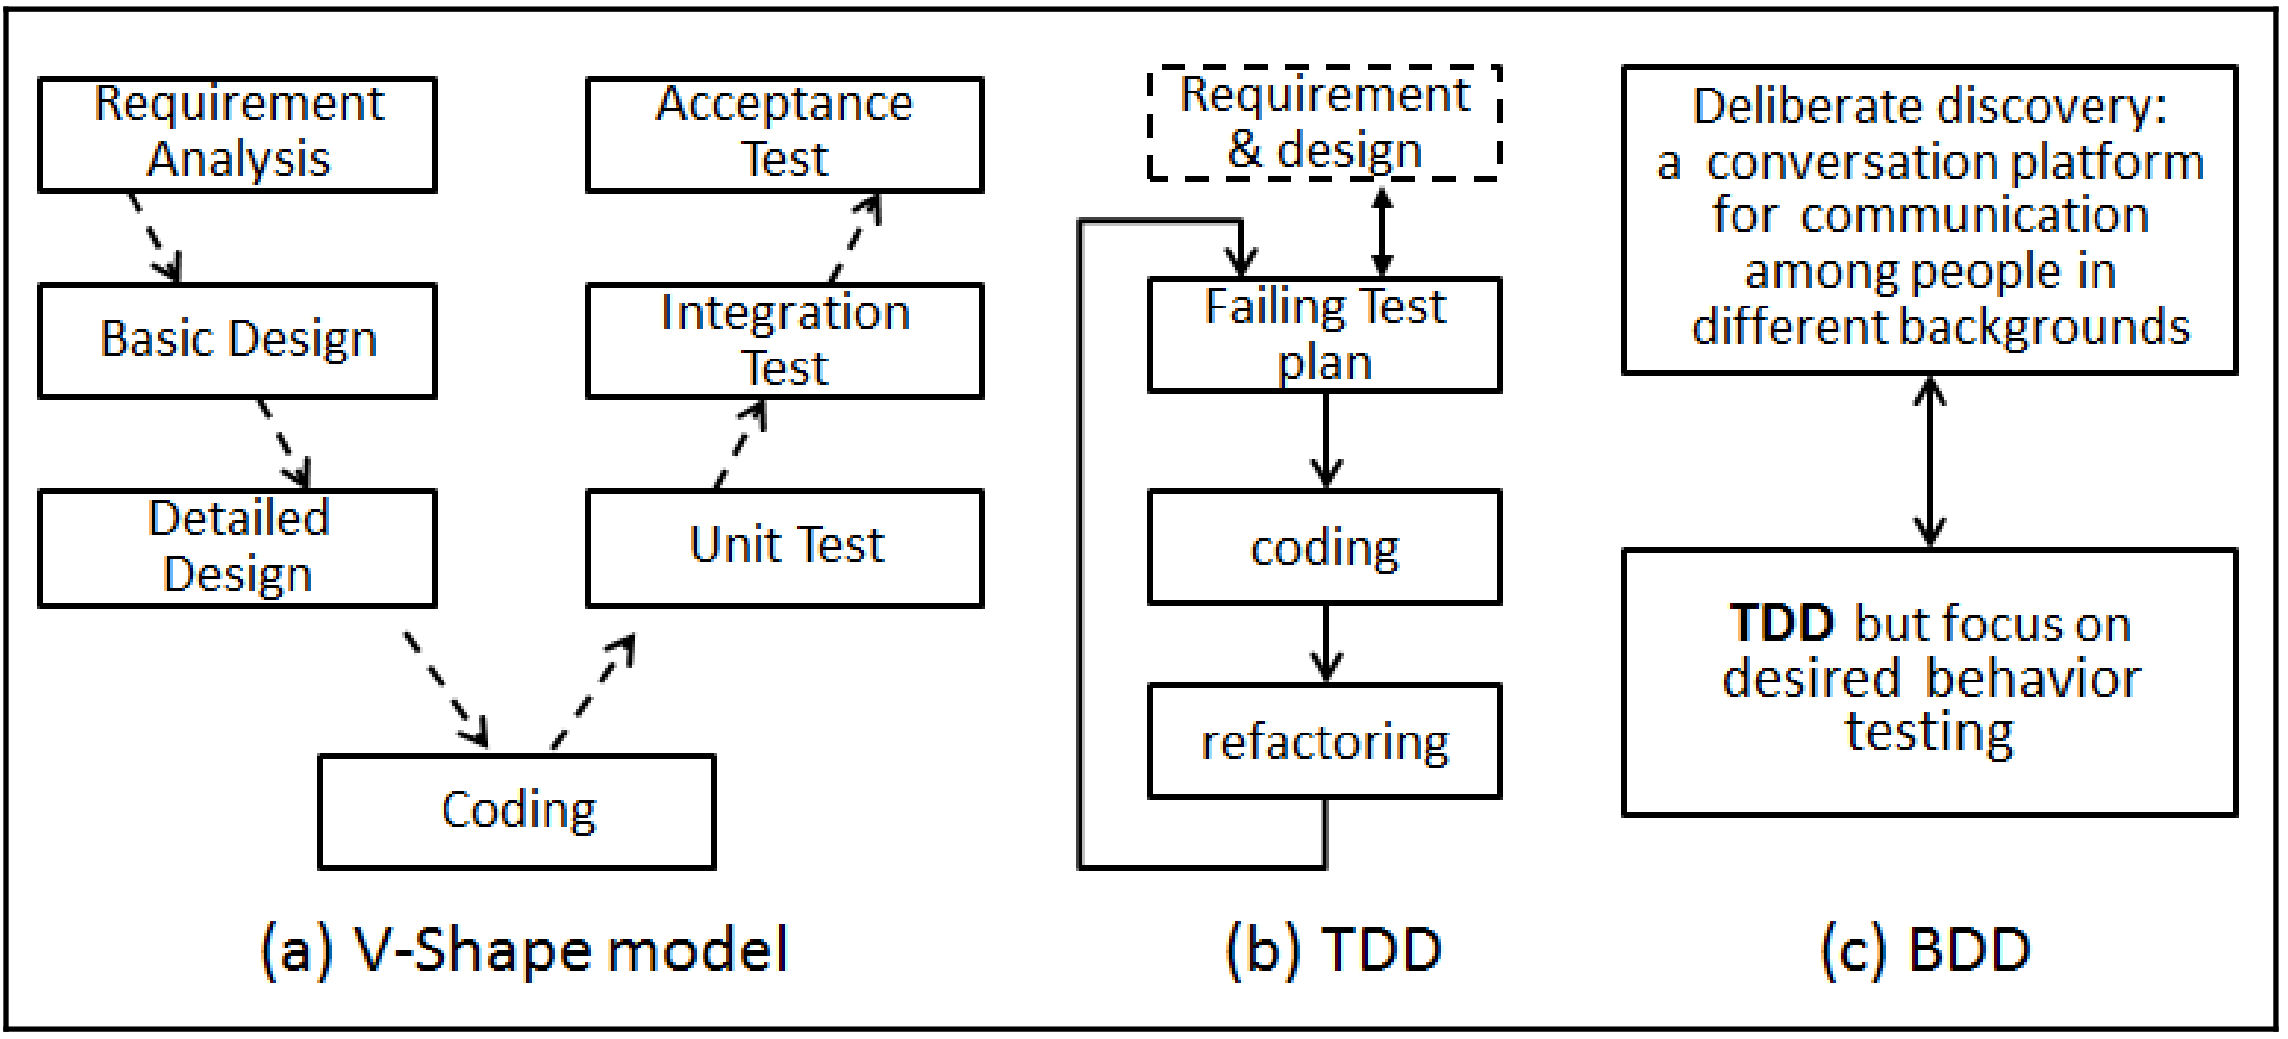
\includegraphics[width=1.0\textwidth]{content/Section-2/Chapter-13/3}
\end{center}

此外,单元测试强调在编码完成时对单个组件进行测试。TDD更侧重于如何在编写代码之前编写测试,然后通过下一个级别的测试计划添加/修改代码。BDD鼓励客户、业务分析人员、开发人员和质量保证分析人员之间的协作。尽管可以单独使用它们,但应该将它们结合起来。 \par

\noindent\textbf{}\ \par
\textbf{总结} \ \par
在本章中,我们简要介绍了软件开发过程中与测试和调试相关的主题。测试可以发现问题,而根本原因分析有助于在宏观层次上定位问题。然而,良好的编程习惯可以在早期阶段防止软件缺陷。此外,称为GDB的命令行接口调试工具,可以帮助我们设置断点并逐行执行程序,同时在程序运行期间打印变量的值。 \par
我们还讨论了自动分析工具和涉及人工测试的过程。静态分析在不执行程序的情况下评估程序的性能。另一方面,动态分析工具可以通过执行程序来发现缺陷。最后,我们了解了在软件开发管道中应该涉及什么、何时以及如何涉及测试过程的策略。单元测试强调在编码完成时对单个组件进行测试。TDD更侧重于如何在开发代码之前编写测试,然后通过下一个级别的测试计划来重复这个过程。BDD鼓励客户、业务分析人员、开发人员和质量保证分析人员之间的协作。 \par
在下一章中,我们将学习如何使用Qt为跨平台应用程序创建图形用户界面(GUI)程序,这些应用程序运行在Linux、Windows、iOS和Android系统上。首先,我们将深入研究跨平台GUI编程的基本概念。然后我们将介绍Qt及其小部件的概述。最后,通过一个案例研究的例子,我们将学习如何使用Qt设计和实现一个网络应用。 \par

\noindent\textbf{}\ \par
\textbf{扩展阅读} \ \par
\begin{itemize}
	\item J. Rooney and L. Vanden Heuvel,  Root Cause Analysis For Beginners , Quality Progress, July 2004, p.45-53.
	\item T. Kataoka, K. Furuto and T. Matsumoto,  The Analyzing Method of Root Causes for Software Problem s, SEI Tech. Rev., no. 73, p. 81, 2011.
	\item K. A. Briski, et al.  Minimizing code defects to improve software quality and lower development costs , IBM Rational Software Analyzer and IBM	Rational PurifyPlus software.
	\item https://www.learncpp.com/cpp-programming/eight-c-programming-mistakes-the-compiler-wont-catch .
	\item B. Stroustrup and H. Sutter, C++ Core Guidelines:  https:/​/​isocpp.​github.​io/CppCoreGuidelines 
\end{itemize}

\noindent\textbf{}\ \par
\textbf{练习和问题} \ \par
\begin{enumerate}
	\item 使用gdb对ch13\underline{ }gdb\underline{ }2.cpp进行断点、条件断点的设置,以及watchpoint,continue和finish命令的使用。
	\item 使用\texttt{g++ -c -Wall - weffc++ -Wextra x.cpp -o x.out}编译cpp文件ch13\underline{ }rca*.cpp。警告中看到了什么?
	\item 为什么静态分析会产生误报,而动态分析不会?
	\item 下载ch13\underline{ }tdd\underline{ }v2.h/.cpp并执行下一阶段的重构。这时,我们将添加复制构造函数、赋值操作符和元素操作符,如+、-、*、/等。具体来说,要做到以下几点:
	\begin{enumerate}
		\item 将第三个测试用例添加到我们的测试套件中,即ch13\underline{ }tdd\underline{ }Boost\underline{ }UTF2.cpp。
		\item 将这些函数的实现添加到文件中,例如:ch13tdd\underline{ }v2.h / . cpp
		\item 运行测试套件进行测试。
	\end{enumerate}
\end{enumerate}

\newpage